% This is samplepaper.tex, a sample chapter demonstrating the
% LLNCS macro package for Springer Computer Science proceedings;
% Version 2.20 of 2017/10/04
%
\documentclass[runningheads]{llncs}
%
\usepackage{graphicx}
\usepackage{dirtytalk}
\usepackage{enumitem}
\usepackage{pifont}
\usepackage{float}
\usepackage{csquotes}

% \usepackage{floatflt}% package for floatingfigure environment

% Used for displaying a sample figure. If possible, figure files should
% be included in EPS format.
%
% If you use the hyperref package, please uncomment the following line
% to display URLs in blue roman font according to Springer's eBook style:
% \renewcommand\UrlFont{\color{blue}\rmfamily}

\begin{document}
% Welche Aufgaben hat unser System? Was brauchen wir für Komponenten zur Realisierung? Wie können wir die sinnvoll in Threads unterteilen?
\title{Final Report: Chinese Whispers}

\author{Group 1: Nadine Bisswang (804957) \and Johannes Deufel (804958) \and Jonas Pfaff (804930) \and Philipp Straub (804934)}

\authorrunning{Group 1: Nadine Bisswang \and Johannes Deufel \and Jonas Pfaff \and Philipp Straub}

\institute{GitHub Repository: \href{https://github.com/Bltzz/Distributed-Systems}}
%
\maketitle              % typeset the header of the contribution
\section{Introduction}
    As part of the Distributed System Project, we implemented the game \say{chinese whispers} (german: \say{Stille Post}) in a distributed system as part of the examination performance. 
    This historical children's game primarily serves the perceptual education of children and is didactically very valuable especially at kindergarten age. The goal of the game is, for all players involved, to correctly pass on a previously selected word or phrase. The attraction of the game (for the kids and educators) results from the fact that the last player has to pronounce what has been passed on aloud -- this often results in very funny misunderstandings. 
    
        \begin{figure}
        \center 
        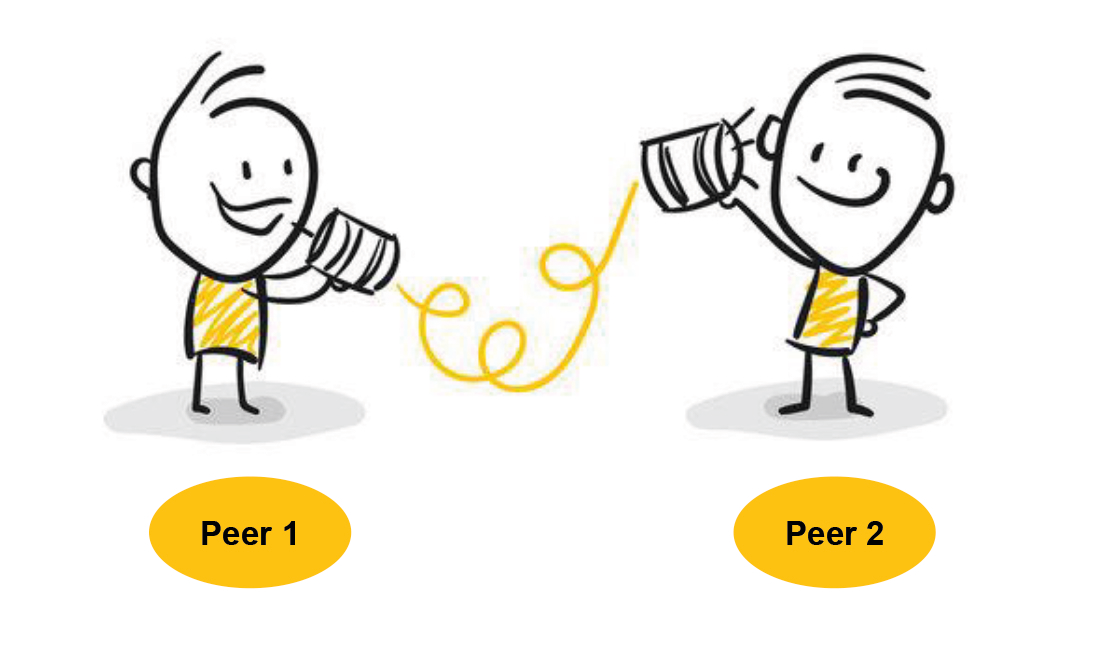
\includegraphics[width=8cm]{Chinese Whispers.pdf}
        \caption{Illustration of the game} \label{fig:chinese-whispers}
        \end{figure}
        
    In the computer-assisted version it must also be possible for individual players to leave the circle, just like in kindergarten. Furthermore, the game must continue if the game leaders (educators) have to move away from the group (or, in IT-terms: crash).
    
    It is very reasonable to map this game within a distributed system, as it is also formed in reality from many, distributed players. Without the distribution or the participation of at least three players, the game is not playable. Furthermore, the system follows a synchronous approach, since - just like in the real game - you have to wait for the previous player to pass on what he understood.
    
\section{Project Design}
    \subsection{Project Structure}
        Our project is separated into three different components: The middleware, the game-logic itself and the main thread. The middleware makes use of UDP and TCP sockets available in python to implement the functionalities of the distributed system and fulfill the three main requirements (dynamic discovery, crash fault tolerance and voting) set for it. As second part, our game-logic makes use of this communication abstraction and ensures the correct procedure. While both middleware and game-logic bring their own functionalities, the only purpose of the main thread is to combine those functionalities, as it is only intend as initiating component of our solution.
    
    \subsection{System Architecture}
        Chinese Whispers is a game with a de-central organization. In the game, participants (the more the better) arrange themselves in a line or circle. All members are of the same kind with one exception. One of these members is the leader. The leader is responsible for one additional task: The definition and passing of the initial word. 
        
        Due to the fact, that in a Peer-to-Peer (P2P) Network various computers work together on an equal level, we decided to choose such a P2P Network for the implementation. This decision is mainly influenced by the original game of chines whispers as there is also no centralized component and the game follows a decentralized approach. Because we have not found any valid arguments against a P2P architecture, we took the game as a pattern for our architecture. The following visualization of the system architecture in Figure \ref{fig:architecture} describes the system behaviour once the game has started and a game leader was elected. This whole behaviour is based on the communication of four different properties via UDP Broadcast or TCP Unicast as shown.
        
        \begin{figure}
            \includegraphics[width=\textwidth]{architecture.pdf}
            \caption{System Architecture} \label{fig:architecture}
        \end{figure}

\section{Requirements -- Addressing \& Implementation}
    \subsection{Requirement 1 -- Dynamic Discovery} \label{sec:dynamic-discovery}
        \subsubsection{Description}
            To enable our solution to be dynamically joined and left, we implement the dynamic discovery of hosts. Within a Peer-to-Peer architecture we see different scenarios how dynamic discovery will appear: 
            \begin{itemize}
                \item A peer starts and a network already exists, 
                \item a peer starts and is the first node of a network or 
                \item a peer is already a node in a network.
            \end{itemize}
            
        \subsubsection{Implementation Details}
            In each of these cases, each peer creates, manages and shares its own group view. However, before any other task is done, each peer creates its own TCP unicast listener and a UDP broadcast listener that run in parallel with threading. Additionally every peer starts its own Hearbeat listener, which, however, does not play an additional role in dynamic discovery. The approach is illustrated in the Figure~\ref{fig:peer-structure} below.
            
            \begin{figure}[H]
           \includegraphics[width=\textwidth]{peer-structure.pdf}
            \caption{Structure of peers} \label{fig:peer-structure}
        \end{figure}
            
            The detailed process stages are listed below.
            \begin{enumerate}
                \item Every peer starts the Unicast Listener first
                \item Then, every peer starts the Broadcast Listener, so that he notices if someone sends broadcast
                \item Afterwards every peer starts the Hearbeat Listener
                \item After all listeners are started, the Broadcast sender is started. Based on a UDP broadcast, each peer then sends a request to join the group (with the initial message with its IP and UUID).
                \item All other peers that are already in the network respond using TCP unicast with their IP and the UUID.
                \item  The TCP Unicast listener of the new host receives these messages, sends an acknowledgement to the other peers and can add them to its own group view.
                \item  Additionally, each peer can add the new joiner to its own group view. 
             \end{enumerate} 
             As we consider a topology of a synchronous uniform non-anonymous ring to be the most suitable for this kind of game (to enable voting), we implemented a logic that allows each peer to find its neighbours.
            Figure \ref{fig:dynamic_discovery} shows the sent messages during the dynamic discovery of new peers and how they are added into the own group view of the member.
        
            \begin{figure}[h]
                \includegraphics[width=\textwidth]{dynamic_dicovery.pdf}
                \caption{Dynamic Discovery} \label{fig:dynamic_discovery}
            \end{figure}
            
            Once enough peers were detected in the game (at least three peers), the meanwhile elected leading peer (see section \ref{sec:voting}) get the option to initiate a start signal by sending a broadcast message to all peers. Then the system starts the game.
        
    \subsection{Requirement 2: Crash fault tolerance} \label{sec:fault-tolerance}
        \subsubsection{Description}
            To ensure that the game is still working once one of the peers crashes, the system must implement crash fault tolerance. Therefore, each peer receives signals from its two neighbours in the ring topology called \enquote{heartbeats}. Those heartbeat messages will be sent through an TCP Unicast. As there is a different error handling needed whether a leader or a peer crashes, we need to handle both scenarios differently. In addition, the current game state affects how an error is handled to ensure that our solution is still playable in the event of a peer crash.
            
            \subsubsection{Implementation Details}
            Our system includes different crash fault tolerance approaches, which are listed below.
            \begin{itemize}
                \item \textbf{Scenario 1: A peer crashes,} the goal is to bring all peers secured into a waiting state until the missing peer joined again, as the game should support the feeling of a team among the players. This will be detected and solved through:
                \begin{itemize}
                    \item \textbf{Missing heartbeat and peer-deletion from the game:} If one peer didn't answer after three times and its heartbeat is missing, the peer which sends the message, can report the absence to the leader to rearrange the topology. In most cases, the rearrangement of the ring should be enough. To rearrange the ring, the current leader informs the active peers that they should delete the missing peer from their list (list with IP and UUID from dynamic discovery). With this updated ring, the peers wait for the lost player to restart the game afterwards.
                    \item \textbf{Missing heartbeat and missing word:} To ensure that no word is lost (even if the peer is down), we store the words in a \enquote{word-history}. Each time the word is passed on, the history is also passed on. However, only the newest word is printed. Even if a peer fails, you can check what the last word was with this history. With that solution, the peer, which lost his neighbour, can track the word history even though it is waiting for the other peer to rejoin. This functionality also enable to handle any misleading user input.
                \end{itemize}
                Depending on the peer's current game state, additional steps are sometimes required to allow to redirect into the waiting state. For example a peer currently awaiting the users input needs to submit the input before getting informed about an crashed peer. So, the just inserted word is therefore not forwarded.
                \item \textbf{Scenario 2: A leader crashes,} the goal is to continue the game undamaged. As the leader is also a normal peer with additional tasks, this builds up on Scenario 1. This will be solved through the peer, which first detected the crashed leader. This peer will take over the leader role temporary, informs the other peers in the ring and then starts the voting (see section~\ref{sec:voting}). Depending on the current game state, this new leader must access one functionality, so the game can continue respectively restart once all peers are complete again.
                \begin{itemize}
                    \item \textbf{The initial word has already been sent by the crashed leader: } The new temporary leader keeps on playing the game like a normal peer, still it needs to change from \enquote{waitForResult} to \enquote{waitForStart} and keeping the leader role at the same time.
                    \item \textbf{The initial word has not been sent by the crashed leader:} The new temporary leader waits until a new leader has been voted. This new leader achieves the leader condition to start a new game once all peers are complete again. The old temporary leader will get revoked its rights to distribute the new starting signal of the game if it is not the new leader.
                \end{itemize}
            \end{itemize}
            
            Although the minimum number of players is 3, the peers need to specify with how many peers to play during the game. This number must be the same for every peer and is therefore the new minimum of playing peers. As described above, the game always takes a break and restarts automatically once the number of players falls below the specified number.
            
    \subsection{Requirement 3: Voting} \label{sec:voting}
        \subsubsection{Description}
            The system must enable initial voting. From this voting a leader emerges, who distributes the points in the game and selects the word from a given list.
            
            In addition, the system must be able to initialize a new voting in case of failure of a peer (if it was the leader) and thus determine a new leader (see section~\ref{sec:fault-tolerance}).
            
        \subsubsection{Implementation details}
            As we are working in a ring topology, we make use of the LaLann-Chang-Roberts algorithm for the leader election. For our case of the \enquote{Chinese Whispers}  Game we adapt the LaLann-Chang-Roberts algorithm and used a self-modified version of that algorithm. The process for the implemented voting is listed below.
            \begin{enumerate}
                \item The voting always starts when a new peer joins the ring initiated by the new joiner
                \item If the systems contains only one peer, this peer is voting with itself
                \item The list of peers is sorted by IP address (info from Dynamic Discovery see section~\ref{sec:dynamic-discovery}). So every peer knows who is its left and who is its right neighbour.
                \item To start the voting process, the leader sends a message to its right neighbour via TCP Unicast. This message contains the UUID from the sender
                \item If the receiving UUID (from the sender) is higher then the UUID from the receiver, the peer (receiver) forwards the message. 
                \item If the UUID from the receiver is higher than the UUID from the sender, the peer (receiver) drops the message and sends an own with its own UUID.
                \item When the message has circulated 1x, we are back at the beginning. This means that we know that there is no one with a higher ID. So with this way the message goes once through the whole ring and ends up at its initial sender with the same UUID. Once this peer receives its own message, it knows, that it is the elected leader.
                \item This elected leader sends the election acknowledgement (message leaderElected = true) via TCP Unicast to its neighbour (right neighbour) which forwards this message until all peers in the group know the leader.
            \end{enumerate}

\section{Application}
    With the implementation of the three above described requirements and the game logic, our distributed system is developed.
    
    To get a better understanding, how the game is working through a distributed system (Peer-to-Peer Network) we listed the game stages below.
    \begin{enumerate}
        \item Game Start: With at least three peers the game is able to start
        \item Every peer starts its Broadcast Listener, Unicast Listener and Heartbeat Listener
        \item If the Hearbeat Listener runs and there are enough peers (three) the game can start
        \item During the game, each game can be in five different stages:
        \begin{itemize}
            \item WaitForStart (initial game state)
            \item InsertWord (Game state while passing the word)
            \item WaitForWord
            \item WaitForResult
            \item ProcessResult
            \item ResetWaitForState
        \end{itemize}
        
        At the beginning all are in the status \enquote{WaitForStart}. If a peer fails, the state \enquote{ResetWaitForState} is used to always trigger the start of a new Game.
        \item Every peer sends its IP and UUID via UDP Broadcast to all participants. Each participant will add the IP and UUID from the sender (peer) to its own list. So every peer in the system knows, who is in the system and the game. As this list is sorted in ascending order by the IP, each peer knows at the end who its neighbours are. 
        \item To check, if the peers are awake, every peer starts its Unicast Sender. That means, that every peer sends a Heartbeat (Unicast) to its right and left neighbour and waits for a response (waiting maximum 3 response times).
        \item The peers (neighbours), which received this heartbeat, answer with the command (cmd) \enquote{awake}.
        \item Then the leader election process will start (see section~\ref{sec:voting}).
        \item After the leader is elected, the leader will select one word from the attached CSV-file and will send this word to its right neighbour via TCP Unicast. Every time a message is sent, the game status of the receiving peer is changed. After sending the 1st word, the status of the sender (leader) changes to \enquote{ProcessResult}. The receiving peer changes to \enquote{InsertWord}.
        \item The peer, which received the message (the word and the word-history) will then insert the understood word.
        \item We have implemented an algorithm that reads a word from the CSV file. With a probability of 33\% the correct word is passed on.
        \item Then the steps 9, 10 and 11 will be repeated. During the game, the presence of the peers is checked (with heartbeats).
        \item When the word reaches 1x in the circle, the game ends. At the end, the list with the history of how the word has changed is displayed.
    \end{enumerate}
    
    To enable parallelism and reduce waiting times, we implement seven types of threads:
    \begin{itemize}
        \item \textbf{Main thread:} Within the main thread, e.g. a broadcast message will be sent
        \item \textbf{Broadcast listener:} This thread is parallel to the main thread. That means, that during the sending of a message from the main thread, the broadcast listener listens the whole time.
        \item \textbf{Unicast listener:} Runs also parallel to the main thread
        \item \textbf{UDP Broadcast Handler:} If a broadcast is received (e.g. current game state), the message will be added to the UDP Broadcast Handler and will be interpreted there. 
        \item \textbf{TCP Unicast Handler:} If a unicast is received (e.g. passed word), the message will be added to the TCP Unicast Handler and will be interpreted there.
        \item \textbf{Heartbeat Listener:} This heartbeats listens to the heartbeats of the right and left neighbours
        \item \textbf{Heartbeat Sender:} This sends the heartbeats and proves the incoming acknowledgements to detect failing peers
    \end{itemize}
    
\section{Summary}
    The goal was to implement the game \enquote{chinese whispers} in a distributed system. For that, we implemented TCP and UDP sockets. The main.py brings all the components of the game together.
    
    With the implemented game we fulfilled the three necessary requirements: (1) Dynamic Discovery (see section~\ref{sec:dynamic-discovery}), (2) Crash fault tolerance (see section~\ref{sec:fault-tolerance}) and (3) Voting (see section~\ref{sec:voting}). In contrast to the real game, we implemented an algorithm to select the word that has been understood from a CSV file. Therefore it is not possible to play our version with your friends interactively, as all peers play on their own.
    
    During our implementation we had several challenges. The biggest challenge was to set up a network with more than one physical/ virtual machine. For example, the virtual machines did not work on a Macbook (newest macOS system). 
    
    As we have progressed in implementing and solving the challenges, we have been able to work together better and better and solve future bugs faster.
    
    To give an outlook, our game could be optimized in the future. It would be better to make a more lightweight implementation and reduce the code. However, our focus within this project was first on the initial implementation of the game logic and necessary requirements. This created foundation now provides a starting point to further optimize the game.

\end{document}